This section describes the methodology that is proposed to be followed during the development of the project.

\subsection{Proposed Software Development Life Cycle}
The project will be developed as per the waterfall model of software development life cycle as depicted in Figure \ref{fig:sdlc}. The reason for choosing this model is the lack of sufficient time duration for agile and iterative methods, as well as very low chances of the changes of requirements in the process of development. 

\begin{figure}[h]
	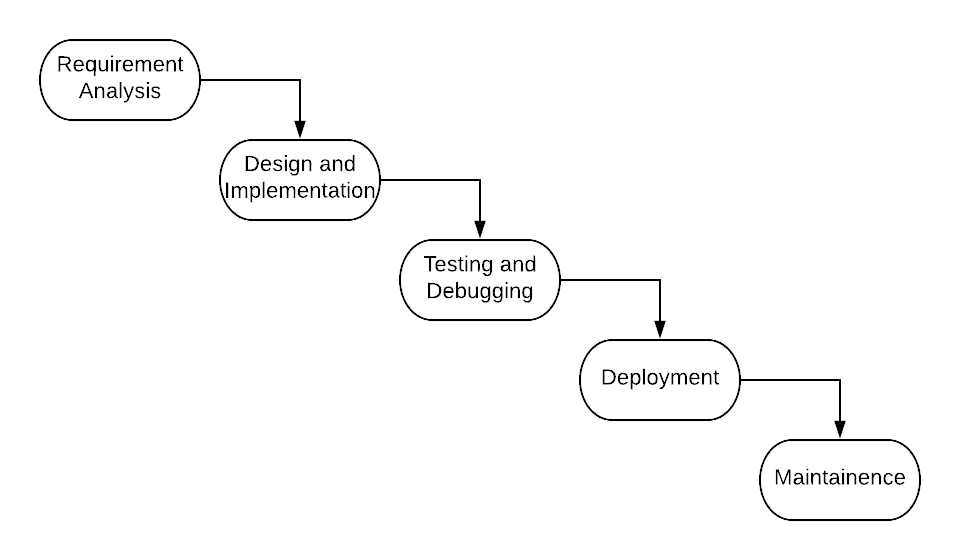
\includegraphics[width=\linewidth]{figures/sdlc.png}
	\centering
	\caption{Proposed software development life cycle}
	\label{fig:sdlc}
\end{figure}

The life cycle begins when the team collects and evaluates the requirements that will be expected from the application. The design and implementation phase will be to design and build both API services and client applications. By the end of this phase, a minimal viable product (MVP) will already have been constructed. In the testing and debugging phases, the quality control methods will be applied to both API and application. Finally, the application will be deployed to Docker containers at the end of the deployment phase. However, there might be slight modifications in the original waterfall model where the design and implementation may be changed slightly after the testing phase if seen reasonable.

\subsection{Technical Architecture}
The application will be built upon the client-server web architecture, as illustrated in Figure \ref{fig:arch}.

\begin{figure}[H]
    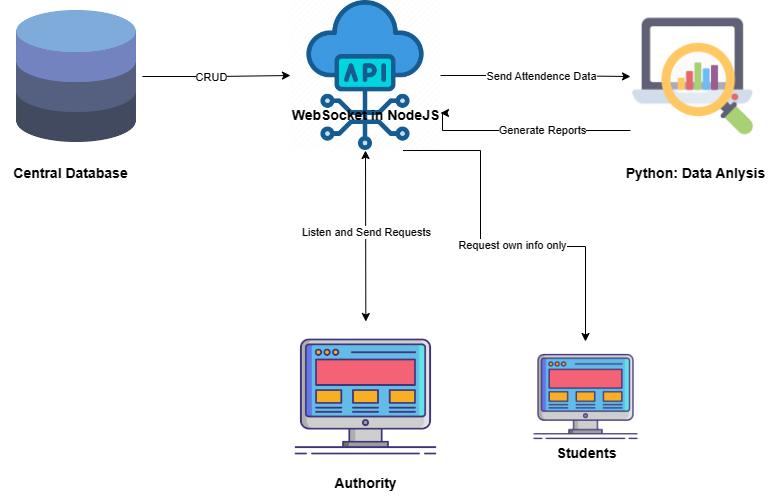
\includegraphics[width=\linewidth]{figures/architecture.png}
    \centering
    \caption{Proposed architecture of the application}
    \label{fig:arch}
\end{figure}

The architecture consists of a database that handles data storage and management. NodeJS, a server-side JavaScript runtime, is responsible for handling Create, Read, Update, and Delete (CRUD) operations on the database. It also provides WebSocket communication capabilities to the client application.\\

The client application allows students to access their personal attendance information securely. Only authorized personnel, such as administrators or instructors, can access the entire dataset via the client application using WebSocket communication.\\

NodeJS acts as the intermediary between the client application and a Python program responsible for generating reports based on the attendance data. This communication ensures seamless integration and efficient report generation.\\

\begin{figure}[H]
    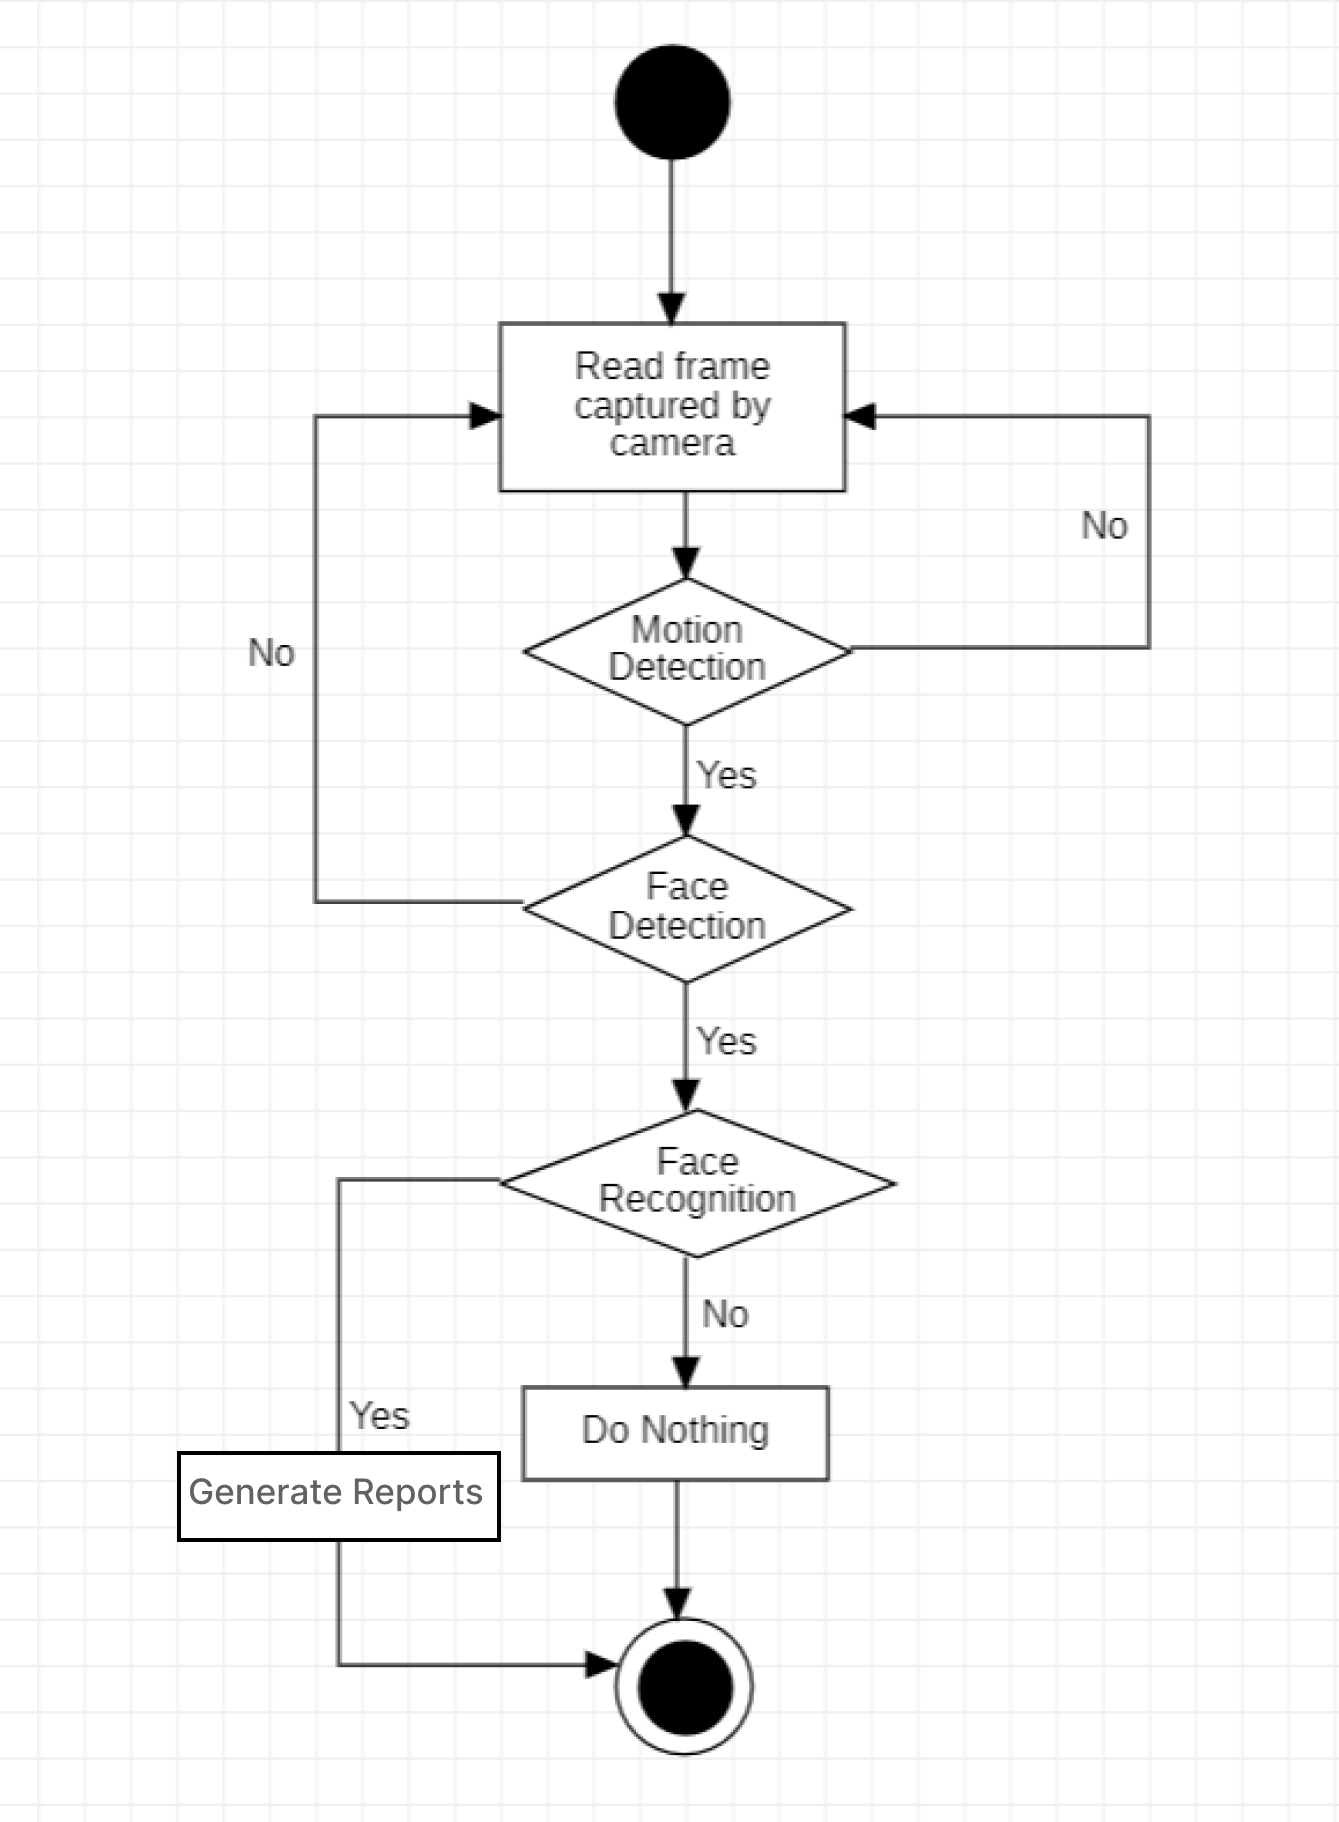
\includegraphics[width=0.6\linewidth]{figures/activity-diagram.png}
    \centering
    \caption{Activity Diagram\cite{yasmeensmart} of the application}
    \label{fig:activity}
\end{figure}

\subsection{Proposed Technologies}
Table \ref{table:tech} consists of the major technologies that are proposed to be used during the development and deployment of the application.

\renewcommand{\arraystretch}{1.5}
\begin{table}[H]
\centering
    \begin{tabular}{|l|l|}
        \hline
        \textbf{Subject}    & \textbf{Proposed Technology} \\ \hline
        Backend Database            & PostgreSQL           \\ \hline
        Backend Service    & Node.js with Express        \\ \hline
        Data Analysis    & Python        \\ \hline
        API Communication & WebSocket \\ \hline
        Frontend(Client)  & Next.js(React), Typescript, TailwindCSS              \\ \hline
        Deployment  & Docker Containers              \\ \hline
    \end{tabular}
    \caption{Technologies proposed to be used}
    \label{table:tech}
\end{table}

